% ----- formatovani dokumentu -----------------------------------------------
\documentclass[12pt,a4paper,titlepage,final]{report}
\usepackage[utf8]{inputenc}
\usepackage[T1, IL2]{fontenc}
\usepackage{graphicx}
\usepackage{epstopdf}
\usepackage[margin=2cm]{caption}
\usepackage[top=3cm, left=2cm, right=2cm, text={17cm, 24cm}, ignorefoot]{geometry}
\usepackage{color}

% ------ commands -----------------------


% ---------------------------------------

\usepackage{url}
\usepackage{setspace}
\singlespacing
\usepackage[square, numbers]{natbib} 
\pagestyle{plain}
\pagenumbering{arabic}
\setcounter{page}{1}

\setlength{\parindent}{1cm}	
\usepackage{natbib}
\renewcommand{\thesection}{\hspace*{-1.0em}}
\renewcommand{\thesubsection}{\arabic{subsection}}



% ----- vyberte jazyk -------------------------------------------------------
\usepackage[english,czech]{babel}
%\usepackage[english]{babel}

% ----- dopiste titulky -----------------------------------------------------
\newcommand\Course{Multimédia}
\newcommand\WorkTitle{Postprocessing OpenGL scény}
\newcommand\AuthorA{Pavel Macenauer}
\newcommand\AuthorB{Jan Bureš}
\newcommand\AuthorAEmail{xmacen02@stud.fit.vutbr.cz}
\newcommand\AuthorBEmail{xbures19@stud.fit.vutbr.cz}
\newcommand\Faculty{Fakulta Informačních Technologií}
\newcommand\School{Vysoké Učení Technické v Brně}

\usepackage[
pdftitle={\WorkTitle},
pdfauthor={\AuthorA\AuthorB},
bookmarks=true,
colorlinks=true,
breaklinks=true,
urlcolor=blue,
citecolor=blue,
linkcolor=blue,
unicode=true,
]
{hyperref}


% ----- titulni strana ------------------------------------------------------

\begin{document}
	\begin{titlepage}
	\begin{center}
		
\includegraphics[height=5cm]{images/logo.eps}
	\end{center}
	\vfill
	\begin{center}
		\begin{Large}
			\Course\\
		\end{Large}
		\bigskip
		\begin{Huge}
			\WorkTitle\\
		\end{Huge}
	\end{center}
	\vfill
	\begin{center}
		\begin{large}
			\today
		\end{large}
	\end{center}
	\vfill
	\begin{flushleft}
		\begin{large}
			\begin{tabular}{lll}
				Autor: & \AuthorA, & \url{\AuthorAEmail} \\
				& \AuthorB, & \url{\AuthorBEmail} \\
		
				& & \\
				& \Faculty \\
				& \School \\
			\end{tabular}
		\end{large}
	\end{flushleft}
\end{titlepage}		

	
% ----- obsah --------------------------------------------------------------
	
\tableofcontents

% ----- obsah -------------------------------------------------------------
\newpage
\section{Cíl projektu}

Cílem projektu bylo vygenerovat OpenGL scénu. Tu následně vyrenderovat do textury, modifikovat pomocí GLSL pixel shaderů a zobrazit. Implementovat různé efekty. Demonstrovat jejich použití na vygenerované scéně. Jednotlivé efekty mělo být možné volit za běhu aplikace.

\section{Popis řešení}

K řešení projektu jsme použili jazyk C++ a vývojové prostředí Visual studio 2012. Pro práci s OpenGL jsme využili knihovny GLUT a GLEW. Samostatné shadery jsou implementovány v jazyce GLSL a každý shader je umístěn v samostatném souboru. Dohromady jsme implementovali 10 shaderů, z toho dva proměnné v čase. Dohromady tedy 10 postprocessing efektů.

\section{OpenGL Framebuffer Object}

Nejvhodnější metodou k renderování do textur v nových verzích OpenGL je využití tzv. Framebuffer Objectu. Samotný OpenGL kontext přichází již s výchozím framebufferem, který se následně využívá k zobrazení na obrazovce, nicméně umožňuje nám vytvořit si i vlastní.

Součástí framebufferu jsou color buffer, depth buffer a stencil buffer. Tyto buffery se musí všechny manuálně alokovat a krom color bufferu jsou nepovinné. Framebuffer umožňuje renderovat i na více lokací naráz a to z toho důvodu, že přehazování samotných framebufferů by byla velmi drahá operace. Max. počet color bufferů je dán grafickou kartou, resp. konstantou \verb|GL_MAX_COLOR_ATTACHMENTS|. 

\begin{center}
	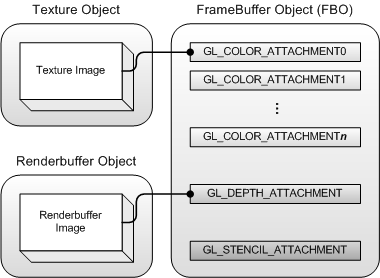
\includegraphics[height=50mm]{images/gl_fbo01.png}
\end{center}

Výhodou vlastního framebufferu je tzv. off-screen rendering, kdy si scénu můžeme vyrenderovat mimo obrazovku do nějaké textury a pracovat pak už pouze ze samotnou texturou. To nachází využití ve 2 oblastech:
\begin{itemize}
	\item postprocessing textury
	\item virtuální pohledy na scénu
\end{itemize}


\section{Jednotlivé funkce shaderů}

K postprocessingu aplikace využívá následujících efektů:

\paragraph{Blur} Rozostření pomocí matice 3x3. Vybere se okolí pixelu na vstupu do shaderu a výsledná hodnota je průměr okolí.

\paragraph{Noční vidění} Převedení obrazu do zeleného spektra.

\paragraph{Černobílá} Převedení obrazu do černobílého spektra.

\paragraph{Inverze} Invertování barev.

\paragraph{Sin} Změna souřadnic pomocí funkce sinus.

\paragraph{Bloom} Jsou zvýrazněny osvětlené plochy a následně rozmazány.

\paragraph{Sobel} Shader na detekci hran pomocí Sobelova operátoru - jak v horizontálním, tak ve vertikálním směru.

\paragraph{Kruhové Vlnění} Kruhové vlnění závislé na čase.

\paragraph{Šum} Šum závislý na čase.

\paragraph{Dithering} Dithering efekt nebo-li redukce počtu barevných složek.

\section{Ovládání aplikace}

Vše potřebné ke spuštění aplikace na platformě Windows je ve složce \verb|exe| a spouští se pomocí \verb|Postprocessing.exe|. Aplikaci je možné ovládat pomocí kláves. Jednotlivé shadery se změní podle stlačené klávesy následovně:

\begin{itemize}
\item 0	Bez efektu.
\item 1	Rozostření scény pomocí matice 3x3.
\item 2	Efekt nočního vidění.
\item 3	Převod do odstínů šedé.
\item 4	Inverze barev.
\item 5	Změna souřadnic texelu pomocí funkce sinus.
\item 6	Zvýraznění odlesků a jejich rozmazání.
\item 7	Detekce hran pomocí sobelova operátoru.
\item 8	Simulace vlnění.
\item 9	Náhodný šum.
\item d Dithering.
\end{itemize}


\section{Galerie implementovaných efektů}

Efekty jsou vykresleny v pořadí jednotlivých stlačitelných kláves viz. Ovládání aplikace.

\begin{center}
\begin{tabular}{lcr}
	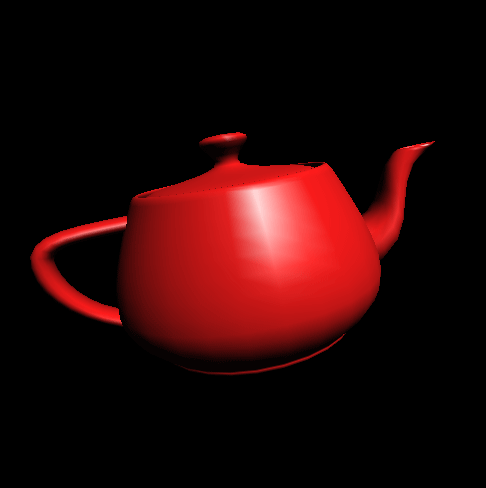
\includegraphics[height=53mm]{images/bezefektu.png} &		
	
\includegraphics[height=53mm]{images/rozmazani.png} &
	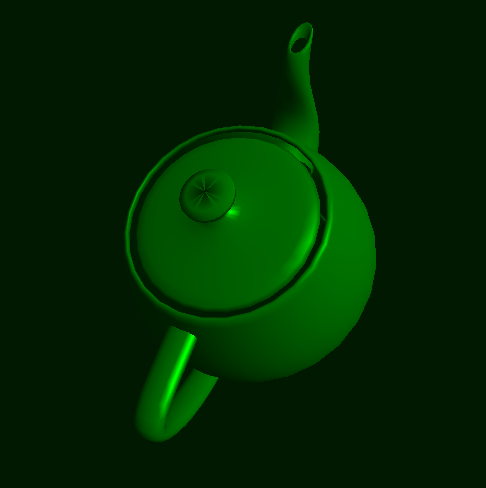
\includegraphics[height=53mm]{images/nightvision.png} \\
	
	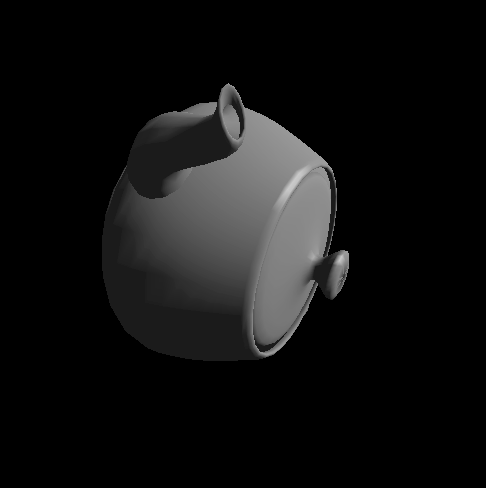
\includegraphics[height=53mm]{images/seda.png} &		
	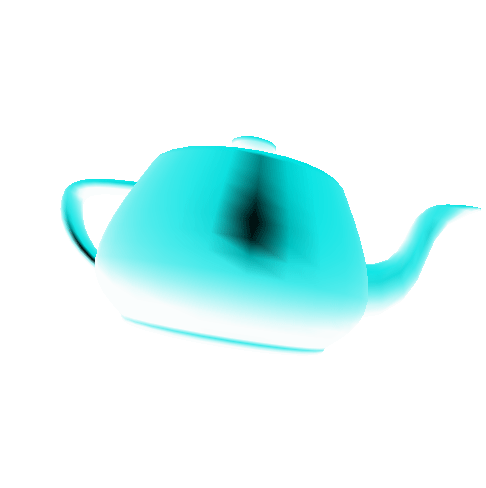
\includegraphics[height=53mm]{images/invert.png} &
	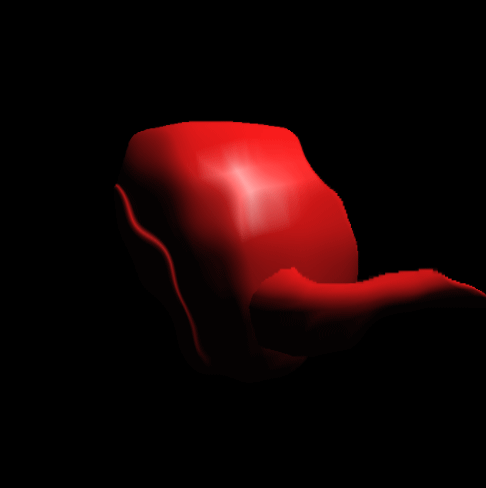
\includegraphics[height=53mm]{images/sin.png} \\
	
	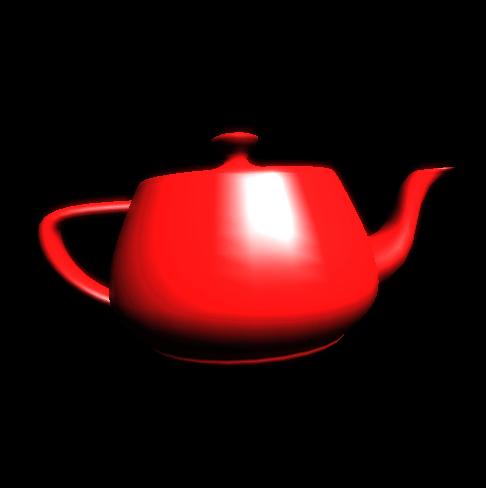
\includegraphics[height=53mm]{images/bloom.png} &		
	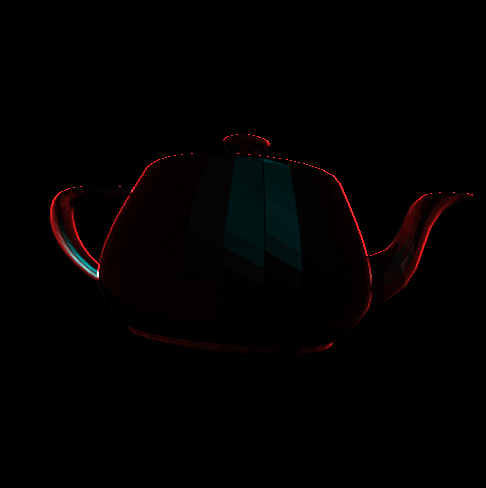
\includegraphics[height=53mm]{images/sobel.png} &
	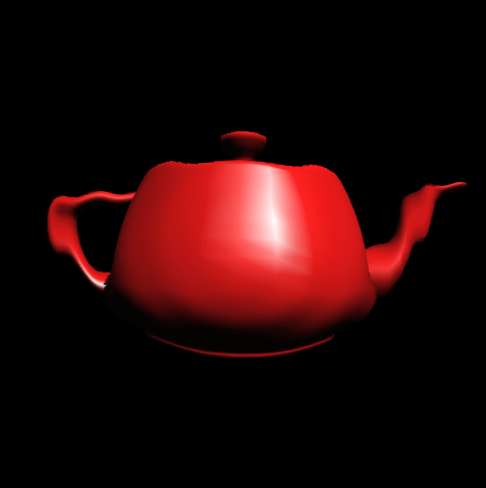
\includegraphics[height=53mm]{images/vlneni.png} \\
	
	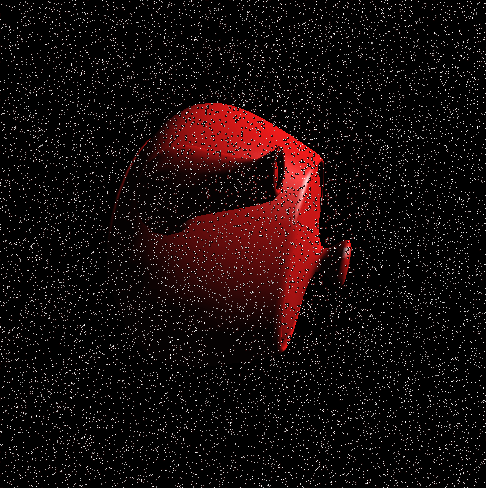
\includegraphics[height=53mm]{images/sum.png} &		
	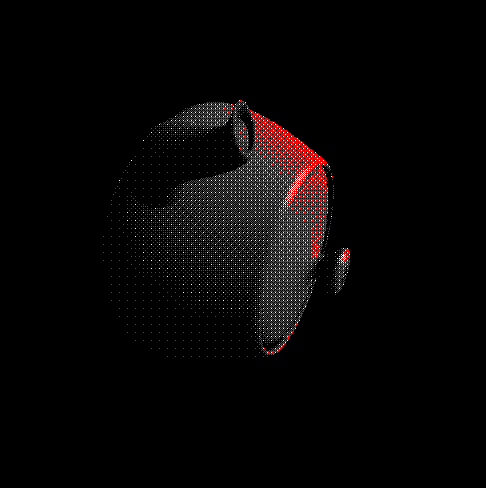
\includegraphics[height=53mm]{images/dithering.png} &
\end{tabular}
\end{center}

\section{Překlad}

Projekt byl vypracován v MS Visual Studiu 2012, je tak dělaný pro platformu Windows. Ve složce \verb|src| je obsažen i projektový soubor, pomocí kterého je projekt preložitelný. Využívá externích knihoven \verb|GLEW| a \verb|GLUT|, které jsou volně ke stažení. Celý projekt je ke stažení na \\
 \url{https://github.com/mmaci/vutbr-fit-mul-postprocessing-opengl} \\
kde jsou přiloženy i všechny potřebné knihovny.




\section{Závěr}

Povedlo se implementovat projekt dle zadání. OpenGL scénou je červený GLUT čajník, který se vyrenderuje do textury a ta je pak vykreslována přes průchod shaderem na obrazovku.

Do budoucna by bylo vhodné implementovat i rozhraní pro řetězení renderování a shaderů (umožňilo by tak fungovat s OpenGL scénu na způsob práce s grafickým editorem, kdy shadery by byly jednotlivé úpravy).

\bibliographystyle{plain}

\nocite{cite1}
\nocite{cite2}
\nocite{cite3}
\nocite{cite4}
\nocite{cite5}

\hypertarget{bib}{}
\bibliography{reference}

\end{document}

